%%%%%%%%%%%%%%%%%%%%%%%%%%%%%%%%%%%%%%%%%%%%%%%%%%%%%%%%%%%%%%%%%%%%%%%%
% Plantilla TFG/TFM
% Escuela Politécnica Superior de la Universidad de Alicante
% Realizado por: Jose Manuel Requena Plens
% Contacto: info@jmrplens.com / Telegram:@jmrplens
%%%%%%%%%%%%%%%%%%%%%%%%%%%%%%%%%%%%%%%%%%%%%%%%%%%%%%%%%%%%%%%%%%%%%%%%

\chapter{Teoría de Antenas}
\par En este capitulo se realizará una breve contextualización sobre el concepto de antena así como un repaso a los parámetros que las caracterizan. Estos conceptos son, por lo general, aplicables a cualquier tipo de antena, en capítulos posteriores se especificará lo aprendido para el caso de las antenas en tecnología microstrip.

\section{Conceptos básicos}

\par Las antenas son transductores entre un medio guaiado y uno radiado. En su diseño más simplificado se analizaría un conductor metálico por el cual fluye una corriente variable en el tiempo. Se entiende como medio guiado a cualquier tipo de línea de transmisión: Cable coaxial, fibra óptica así como guías de onda. Y como medio radiado el aire o el espacio. Las antenas transmisoras serán las encargadas de transformar esta las corrientes eléctricas a \gls{oem}, mientras que las receptoras tomarán las \gls{oem} desde el medio radiado y las convertirán de nuevo a impulsos eléctricos para su posterior procesado. Las primeras antenas fueron diseñadas en 1888 por \textit{Heinrich Hertz} pero no fue hasta 1895 cuando \textit{Guglielmo Marconi} empezó a desarrollar antenas con el objetivo de transmitir información a largas distancias.
\\
\par Como se explico en el capítulo \ref{cap1}, cualquier variación de un campo eléctrico generará un campo magnético y viceversa. Cuando ambos campos conviven y existen variaciones de estos campos se dice que existe una radiación electromagnética. Para entender el principio de funcionamiento de una antena se tomará como ejemplo el caso de hilo conductor cerrado. Si se introdujera una corriente eléctrica fluctuante en el tiempo dentro del conductor, por el principio de inducción electromagnética (Tercera ecuación de Maxwell, Ley de Faraday-Lentz) se produciría un campo magnético fluctuante y un campo eléctrico asociado a su alrededor, estaríamos hablando de un campo electromagnético. Pero este campo electromagnético no se propagaría y estaría siempre al rededor del conductor cerrado. Para poder propagar las \gls{oem} se debe conseguir separar la onda electromagnética del conductor.
\\
\par Para entender el efecto de separación se tomará como referencia dos cargas eléctricas de distintas polaridades separadas a una distancia determinada (fig. \ref{fig:campo1}), a esto se le conoce como dipolo eléctrico y producirán un campo eléctrico cuyas líneas de fuerza irán del positivo al negativo. Estás dos cargas intentarán juntarse debido al efecto de atracción. En el momento de mayor separación de las cargas, su velocidad será nula y su aceleración máxima. Conforme se vayan acercando la velocidad irá aumentando y la aceleración disminuyendo hasta que en el punto donde se encuentran la velocidad será máxima y la aceleración nula. Suponiendo un escenario teórico sin pérdidas estás cargas estarían fluctuando e intercambiando sus posiciones indefinidamente. Si se analiza el campo eléctrico producido por las cargas mientras estas están fluctuando se observaría como, en vez de seguir encontrando un campo eléctrico simple de menor intensidad, este se deforma debido a la aceleración presente en las cargas. Esta deformación es también conocida como efecto \textit{kink} (fig. \ref{fig:campo2}).
\\
\par Continuando con el experimento se observa como pasado un lapso de un 1/4 del periodo de la oscilación, momento en el que las dos cargas se cruzan en el mismo punto, el campo eléctrico producido es nulo, cerrándose así las líneas de campo que habían sido producidas cuando las partículas estaban aún separadas (fig. \ref{fig:campo3}). Es entonces cuando se produce la propagación y generación del frente de onda del campo eléctrico, con su respectivo campo magnético asociado. Se debe observar como la longitud de la \gls{oem} propagada es exactamente el doble de la longitud existente entre las dos cargas (fig. \ref{fig:campo4}).\\

\begin{figure}[h]
\centering
	\begin{subfigure}[b]{0.3\textwidth} % Espacio horizontal ocupado por la subfigura
		\centering
		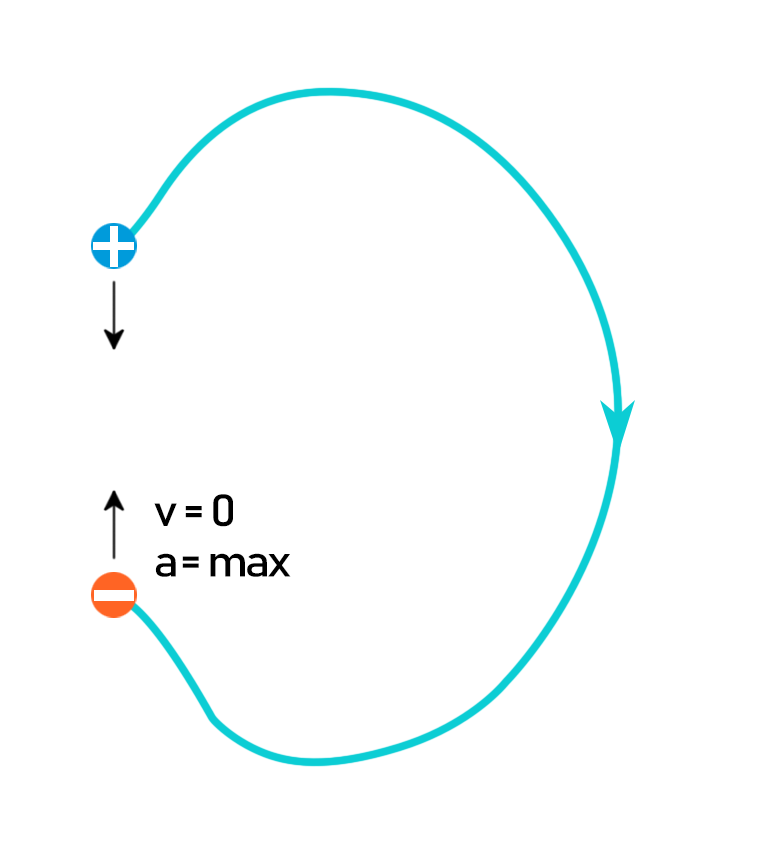
\includegraphics[width=5cm]{archivos/campos/campos1} % Tamaño de la imagen
		\caption{t = 0}
		\label{fig:campo1}
	\end{subfigure}
~ % Añadir el espacio deseado, si se deja la linea en blanco la siguiente subfigura ira en una nueva linea
	\begin{subfigure}[b]{0.3\textwidth} % Espacio horizontal ocupado por la subfigura
	\centering
		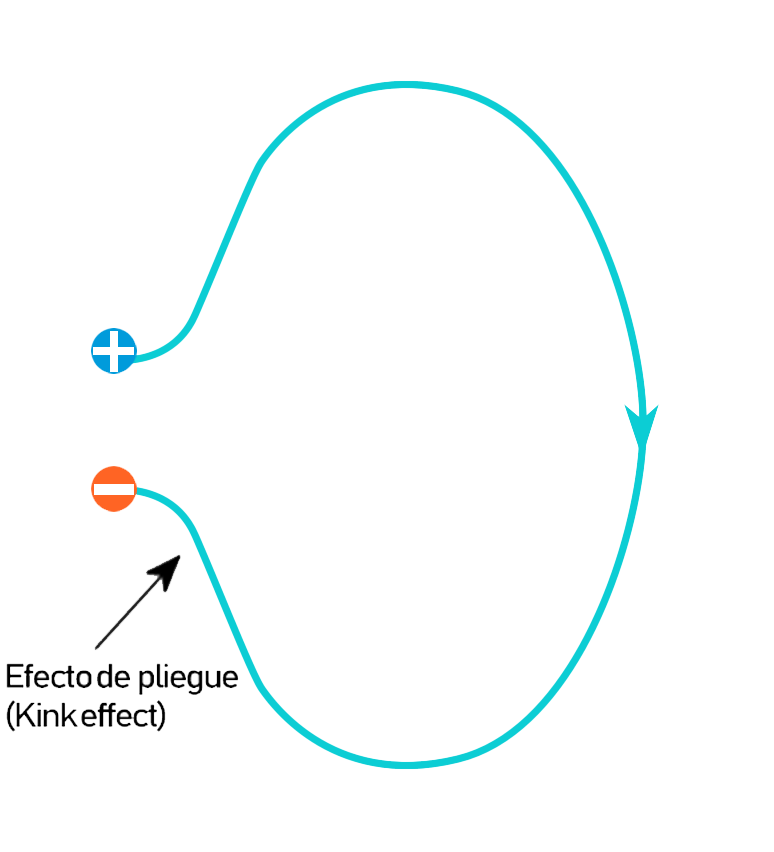
\includegraphics[width=5cm]{archivos/campos/campos2} % Tamaño de la imagen
		\caption{0 < t < T/4}
		\label{fig:campo2}
	\end{subfigure}
	\begin{subfigure}[b]{0.3\textwidth} % Espacio horizontal ocupado por la subfigura
	\centering
		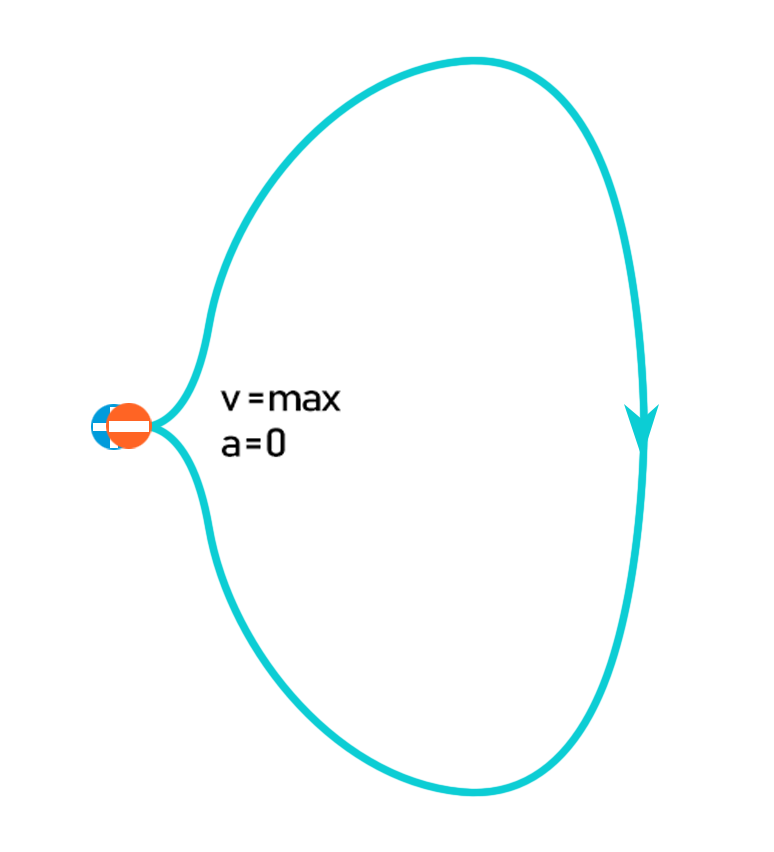
\includegraphics[width=5cm]{archivos/campos/campos3} % Tamaño de la imagen
		\caption{t = T/4}
		\label{fig:campo3}
	\end{subfigure}
	\begin{subfigure}[h]{0.5\textwidth} % Espacio horizontal ocupado por la subfigura
	\centering
	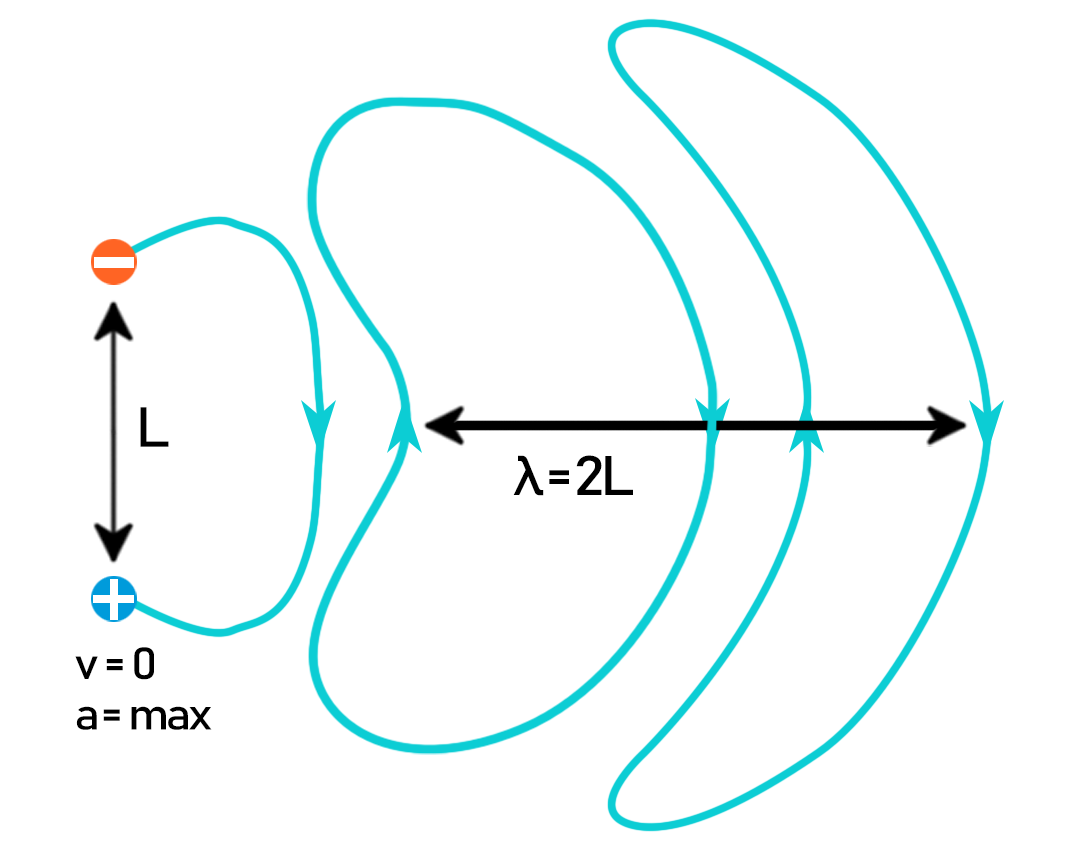
\includegraphics[width=10cm]{archivos/campos/campos4} % Tamaño de la imagen
	\caption{t > T/4}
	\label{fig:campo4}
\end{subfigure}
\caption{Proceso de separación de campo eléctrico}\label{sistemass}
\end{figure}

\par En la práctica se puede simular el experimento en lo que se denomina como antena dipolo, la antena más básica existente, que será estudiada con mayor detenimiento a lo largo de este capítulo. En una antena dipolo, al aplicar una tensión variable sobre los bornes de esta, las cargas irán oscilando de un extremo a otro según la polaridad del generador en ese instante, produciendo campos eléctricos capaces de separarse de la antena, con su consiguiente generación de campos magnéticos. El conjunto de la propagación de ambos campos son los campos electromagnéticos en los que se propagará la \gls{oem}. En la figura \ref{fig:dipolo} se pueden observar ejemplos de antenas dipolo. 

\begin{figure}[h]
\centering
	\begin{subfigure}[b]{0.4\textwidth} % Espacio horizontal ocupado por la subfigura
		\centering
		\includegraphics[width=7cm]{archivos/dipolo/dipole1} % Tamaño de la imagen
		\caption{Esquema de un dipolo}
		\label{fig:dipolo1}
	\end{subfigure}
~ % Añadir el espacio deseado, si se deja la linea en blanco la siguiente subfigura ira en una nueva linea
	\begin{subfigure}[b]{0.4\textwidth} % Espacio horizontal ocupado por la subfigura
	\centering
		\includegraphics[width=7cm]{archivos/dipolo/dipole2} % Tamaño de la imagen
		\caption{Dipolo instalado sobre un poste. \citep{Sirio2012}}
		\label{fig:dipolo2}
	\end{subfigure}
\caption{Antenas dipolo de media onda}\label{fig:dipolo}
\end{figure}

\par El principio básico de diseño de antenas se basa en la geometría de estas. Es importante remarcar que para que la transmisión de la señal aplicada por el generador y que se desea convertir en \gls{oem}, la longitud de los lados del dipolo deben estar relacionados con la longitud de onda de la señal que se desea transmitir. En el caso del dipolo, los extremos tendrán una longitud de $\lambda$/4. Al juntan ambos extremos se puede observar que la antena tendrá una dimensión total de $\lambda$/2, y si se tiene en cuenta que la longitud de onda de la \gls{oem} generada es el doble de la longitud de la antena, se obtendrá una \gls{oem} radiada cuya frecuencia sea idéntica a la aplicada por el generador.
\\
\par Aunque se ha analizado el caso de una antena para que funcione como transmisora, el mismo principio de funcionamiento se aplica cuando queremos que esta funcione como receptora de señales. Una \gls{oem} que viaje por el espacio será capaz de hacer oscilar las cargas de una antena receptora cuando su frecuencia y las longitud de la antena estén directamente relacionadas y se produzca la resonancia sobre esta. La diferencia es que a la salida de la antena receptora no tendremos un generador, sino lo que denominaremos como carga, pudiendo ser esta cualquier tipo de componente eléctrico o electrónico que sea capaz de trabajar con las corrientes eléctricas producidas por la fluctuación de cargas eléctricas en el interior de la antena.

\section{Caracterización de antenas}
\par Para saber qué tipo de antena se puede hacer más conveniente para un uso concreto se ha de tener en cuenta sus características. Las principales características de las antenas son:

\subsection{Polarización}
\par Como se hizo mención en el capítulo \ref{cap1}, las \gls{oem} pueden estar polarizadas. Si se secciona a una \gls{oem} perpendicularmente a su vector de propagación y vemos el dibujo que va formando campo eléctrico en dicha sección conforme pasa el tiempo observaríamos qué tipo de polarización tiene la \gls{oem}. Las tres polarizaciones más comunes son: Lineal, circular y elíptica.

\begin{itemize}
\item\textbf{Polarización lineal: }Cuando se observa que la figura trazada por el campo eléctrico es una recta, se dirá que esta está polarizada linealmente. Analíticamente se producirá polarización lineal cuando las fases de las componentes ortogonales del campo eléctrico difieran en un múltiplo entero de $\pi$ radianes. La variación temporal de los campos eléctricos con polarización lineal se puede representar fasorialmente como:
\begin{equation}
	\vec{E} = \hat{x}e^{^{j(\omega t-kz)}}
	\label{eq:pollineal}
\end{equation}
\begin{figure}[H]
    \centering
        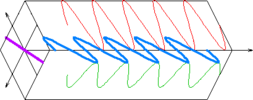
\includegraphics[width=6cm]{archivos/polarizacion/lineal}
        \caption{Onda electromagnética polarizada linealmente}
        \label{fig:pollin}
\end{figure}
\item\textbf{Polarización circular: }Cuando se observa que la figura trazada por el campo eléctrico es un círculo, se dirá que esta está polarizada circularmente. Analíticamente se producirá polarización circular cuando las fases de las componentes ortogonales del campo eléctrico sean $\pi$/2 o 3$\pi$/2 y las amplitudes sean iguales. La variación temporal de los campos eléctricos con polarización circular se puede representar fasorialmente como:

\begin{subequations}
	\begin{eqnarray}
		\vec{E} = (\hat{x}+j\hat{y})e^{^{j(\omega t-kz)}} \label{ecu:polcirlev} \\ % Salto de línea
		\vec{E} = (\hat{x}-j\hat{y})e^{^{j(\omega t-kz)}} \label{ecu:polcirdex} 
	\end{eqnarray}
\end{subequations}

\begin{figure}[H]
    \centering
        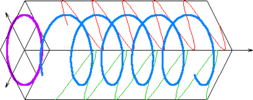
\includegraphics[width=6cm]{archivos/polarizacion/circular}
        \caption{Onda electromagnética polarizada circularmente}
        \label{fig:polcir}
\end{figure}

En este caso el signo que se encuentra en el interior de la suma de componentes indicará el sentido de giro en la polarización circular: Positivo será una rotación levógira y negativo una rotación dextrógira.

\item\textbf{Polarización elíptica: }Cuando se observa que la figura trazada por el campo eléctrico es una elipse, se dirá que esta está polarizada elípticamente. El resto de casos en los que la polarización no sea ni circular ni lineal serán polarizaciónes elípticas. La variación temporal de los campos eléctricos con polarización elíptica se puede representar fasorialmente como:

\begin{equation}
	\vec{E} = ((2+j)\hat{x}-3j\hat{y})e^{^{j(\omega t-kz)}}
	\label{eq:polelip}
\end{equation}
\begin{figure}[H]
    \centering
        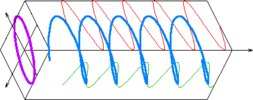
\includegraphics[width=6cm]{archivos/polarizacion/eliptica}
        \caption{Onda electromagnética polarizada elípticamente}
        \label{fig:poleli}
\end{figure}

\end{itemize}

\par En las ámbito de las radiocomunicaciones y en concreto de la telefonía móvil, la polarización más común en la que se emiten y reciben las \gls{oem} es la lineal-vertical. En otros casos como la transmisión de televisión se uriliza polarización lineal-horizontal. En comunicaciones vía satélite se alternan las polarizaciones lineales horizontales y verticales para reducir la interferencia entre señales que transmiten en el mismo rango de frecuencias.
\\
\par Se ha de tener en cuenta que cada antena se diseña para trabajar con una polarización concreta y las señales recibidas cuya polarización sea distinta a esta serán atenuadas debido al \textit{factor de pérdidas por polarización} ($C_{p}$):

\begin{equation}
	C_{p}=\left | \hat{u}_{tx}\cdot \hat{u}_{rx} \right |
	\label{eq:polarizationlossfactor}
\end{equation}

\par Donde $\hat{u}_{tx}$ es el vector unitario del campo eléctrico incidente y $\hat{u}_{rx}$ es el vector unitario del campo eléctrico de la antena receptora. 

\subsection{Impedancia}

\par Cualquier antenas se puede expresar como una carga en un circuito eléctrico, lo que facilita su análisis de impedancias, potencias y adaptación (fig. \ref{fig:impedancia}). Existen varios parámetros de impedancia que caracterizan a la antena. Por lo general, teniendo en cuenta la \textit{Ley de Ohm}, se define la impedancia de una antena como la relación entre la tensión y la corriente en los bornes de esta. 

\begin{equation}
	Z_{a}=\frac{V_{i}}{I_{i}}=R_{a}+jX_{a}
	\label{eq:impendaciaantena}
\end{equation}

\par Donde $R_{a}$ es la componente real u óhmica de la impedancia y $jX_{a}$ es la parte imaginaria o reactiva de la impedancia. La componente real puede ser a su vez descompuesta en dos términos: La resistencia de radiación y la resistencia óhmica o de pérdidas. La resistencia de radiación se define como la relación entre la potencia total radiada y la corriente eficaz en los terminales de la antena al cuadrado. La resistencia ohmica de la antena se define como la relación entre la potencia disipada debido a las pérdidas resistivas y la corriente que circula por sus terminales al cuadrado. Por otro lado la parte reactiva de la impedancia dependerá de sus dimensiones, la frecuencia de resonancia o el tipo de antena que estemos usando.

\begin{equation}
	Z_{a}=(R_{r}+R_{\Omega})+jX_{a}
	\label{eq:impendaciaantenatotal}
\end{equation}

\par Si se analizan las potencias según el tipo de resistencia, de radiación y óhmica, se obtiene que:

\begin{subequations}
	\begin{eqnarray}
		P_{r}=\frac{1}{2}\left | I_{o}  \right |^{2}R_{r} \label{ecu:potenciarad} \\ % Salto de línea
		P_{\Omega}=\frac{1}{2}\left | I_{o}  \right |^{2}R_{\Omega} \label{ecu:potenciaohm} 
	\end{eqnarray}
\end{subequations}

\begin{figure}[h]
    \centering
        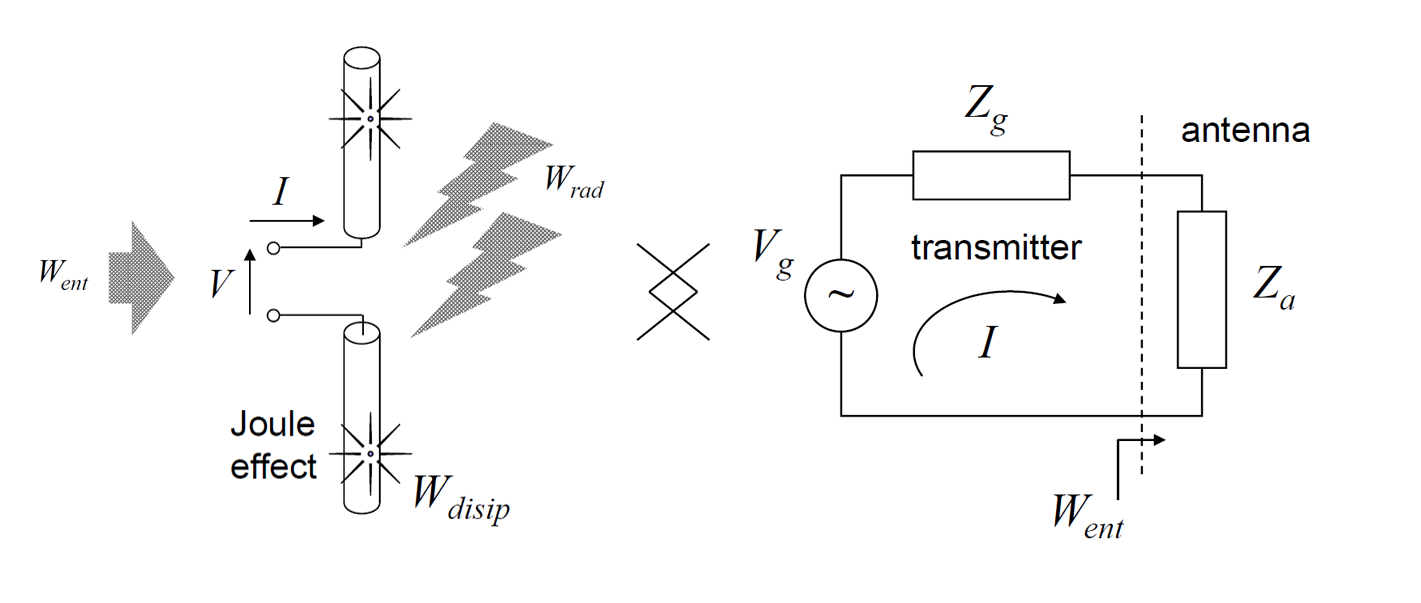
\includegraphics[width=15cm]{archivos/impedancia}
        \caption{Circuito equivalente de una antena transmisora}
        \label{fig:impedancia}
\end{figure}
\todo{referencia}
\par Otro concepto importante es la denominada adaptación de impedancias. Para que las pérdidas de la antena sean mínimas y conseguir así una máxima transferencia de potencia entre las líneas de transmisión y la antena es importante que las impedancias de cada sistema conectado sean iguales. Cuando las impedancias de nuestros circuitos difieren se pueden producir réplicas o ecos que se reflejan en el sistema entrante e interfieren con la señal que intenta propagarse por la línea de transmisión. Para solucionarlo se debe recurrir a métodos de adaptación como transformadores $\lambda$/4 o circuitos en serie o stub.

\subsection{Diagrama de Radiación}

\par El diagrama de radiación es usado para representar gráficamente las propiedades de la radiación de una antena en un función de unas coordenadas angulares espacias, a una distancia fija. Para su representación se usan coordenadas esféricas o polares. Es una manera muy efectiva de conocer en qué direcciones concentra su radiación nuestra antena así como posibles radiaciones no deseadas que puedan existir un diseño particular. Para representar sobre un plano polar el diagrama de radiación aplicaremos la siguiente ecuación:

\begin{equation}
	t(\theta, \phi )=\frac{\left | E(r, \theta, \phi ) \right |^2}{\left | E_{max}(r) \right |^2}= \frac{P(r,\theta ,\phi)}{P_{max}(r)}
	\label{eq:diagramarad}
\end{equation}

\par El consistir en un plano de dos dimensiones: Angulo de radiación ($\theta$) e intensidad de radiación (t($\theta $, $\phi $)), debemos tener en cuenta que solo obtendremos el diagrama de radiación para un solo ángulo de transmisión de la antena. Es mediante el ángulo $\phi $ con el que podremos ir variando los resultados en el diagrama de radiación para poder observar como se propaga la antena en diferentes planos como son comúnmente el plano E y H (fig. \ref{fig:pattern}).

\begin{itemize}
\item \textbf{Plano E: }Es el plano donde podemos encontrar el vector del campo eléctrico y su dirección de máxima radiación (XZ). Este plano se encuentra en $\phi $ = 0º. 

\item \textbf{Plano E: }Es el plano donde podemos encontrar el vector del campo magnético y su dirección de máxima radiación (XY). Este plano se encuentra en $\phi $ = 90º.
\end{itemize}

\begin{figure}[h]
    \centering
        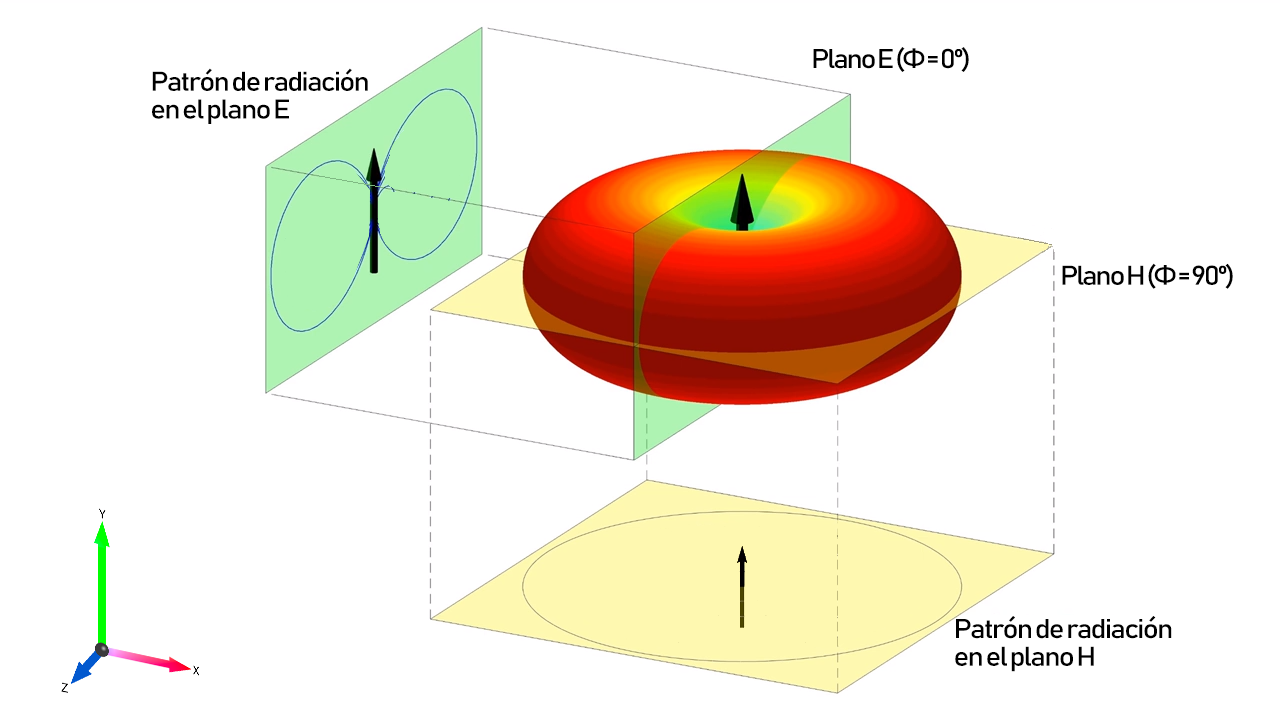
\includegraphics[width=15cm]{archivos/radiacion/pattern2}
        \caption{Ejemplo de patrones de radiación en los planos E y H para antena dipolo. \citep{Yavuz2015}}
        \label{fig:pattern}
\end{figure}

\par Existen ciertos parámetros que caracterizan a una antena que pueden ser localizados y calculados con facilidad gracias al diagrama de radiación tanto en coordenadas polares como en cartesianas (fig. \ref{fig:carte}). Estos parámetros son:

\begin{itemize}

\item \textbf{Lóbulos: }Son los haces de radiación. Se dividen en:
	\begin{itemize}
	\item \textbf{Lóbulo principal: }Se define siempre como la dirección de máxima radiación, siendo este siempre el haz con mayor intensidad de radiación.
	\item \textbf{Lóbulos secundarios: }Son los primeros haces de menor intensidad que aparecen en los laterales del lóbulo principal. 
	\item \textbf{Lóbulos menores: }Son el resto de haces de radiación los cuales son, normalmente, indeseados. Cuanto más directiva sea la antena, mayor será su número. 
	\item \textbf{Lóbulos trasero: }Es el haz de radiación que encontraremos siempre a 180º respecto al lóbulo principal. Normalmente, suele ser indeseado y su presencia puede producir interferencia con otras antenas del entorno así como una menor eficiencia para el propósito de nuestra antena.
	\end{itemize}	

\item \textbf{Ancho de haz a -3dB (HPBW)}: Se define como el ángulo recorrido por el lóbulo principal desde sus dos pasadas por -3dB de potencia, es decir, la mitad de la potencia máxima radiada. 

\item \textbf{Ancho de haz entre nulos (FNBW)}: Ángulo recorrido desde los dos nulos localizados a los laterales del lóbulo principal.

\item \textbf{Nivel de lóbulos laterales (SLL)}: Se define como la diferencia de niveles entre el nivel del lóbulo principal y el primer lóbulo secundario.

\item \textbf{Relación delante/atras (F/B)}: Diferencia de niveles entre el lóbulo principal y el trasero: 

\begin{equation}
	F/B(dB)=-10\log_{10}t(\theta+180^{\circ})
	\label{eq:fb}
\end{equation}

\end{itemize}

\begin{figure}[h]
    \centering
        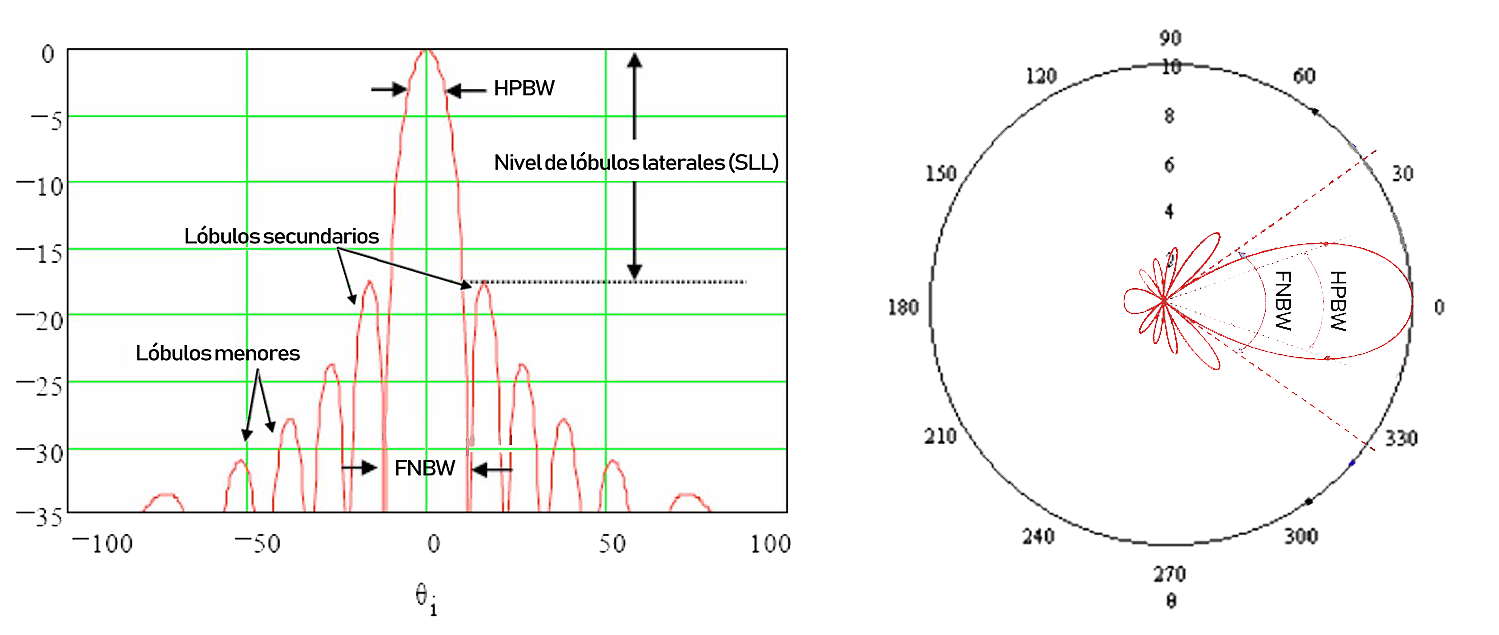
\includegraphics[width=16cm]{archivos/radiacion/pat3}
        \caption{Comparación de los parámetros del diagrama de radiación en planos cartesianos y polares }
        \label{fig:carte}
\end{figure}
\todo{referencia}
\par Los patrones principales de radiación son:

\begin{itemize}
\item \textbf{Isotrópico: }La radiación de la antena fluye en todas las direcciones del espacio. Esta antena es completamente teórica ya que es imposible simular su patrón de directividad en una antena real. Se tiene como referencia para el cálculo de directividad de una antena.
\item \textbf{Omnidireccional: }Se dice que la antena es omnidireccional cuando el patrón de radiación es simétrico y equidistante en todos los ángulos del plano para uno o varios planos de radiación.
\item \textbf{Directiva: }Una antena es directiva cuando uno o varios de sus haces destacan sobre los demás. Esto puede ocurrir de manera intencionada, donde buscamos que el haz apunte hacia una dirección concreta, ej: Radioenlaces. O involuntariamente, cuando por ejemplo, tenemos lóbulos traseros o secundarios de bastante intensidad radiando a la vez que el principal. 
\end{itemize}

\begin{figure}[h]
    \centering
        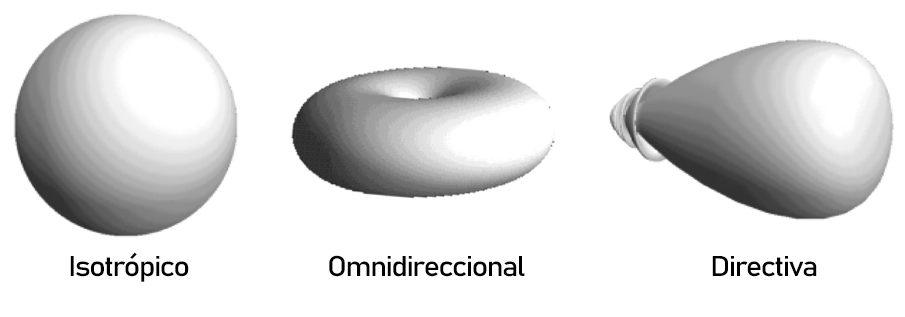
\includegraphics[width=15cm]{archivos/radiacion/patrones}
        \caption{Principales patrones de radiación }
        \label{fig:prinrad}
\end{figure}
\todo{referencia}
\subsection{Directividad}

\par La directividad de una antena se define como la relación entre la intensidad de potencia de radiación en una dirección y distancia concretas, y la misma potencia radiada en caso de que la antena fuera isotrópica, es decir, cuya potencia radiada sea igual en todas las direcciones del espacio (eq. \ref{eq:directividad}). Este parámetro es muy importante para caracterizar la antena ya que representa la capacidad de una antena para concentrar la intensidad de radiación en una dirección determinada. Es posible obtener analíticamente el valor de directividad para un ángulo completo en el plano polar mediante:

\begin{equation}
	D(\theta, \phi )=\frac{P(r,\theta ,\phi)}{P_{iso}}= \frac{P(r,\theta ,\phi)}{\frac{W_{rad}}{4\pi r^{2}}}
	\label{eq:directividad}
\end{equation}

\par Si se observa en el patrón de radiación de una antena, se dirá que esta es más directiva cuanto mayor sea el nivel de intensidad de un haz así como menor sea la anchura del mismo. Para el caso de las antenas directivas (D > 20dB), se puede obtener una directividad considerando que la radiación es uniforme sobre el ángulo sólido definido sobre el HPBW (Ancho de haz a -3dB) mediante la aproximación:

\begin{equation}
	D=\frac{4\pi}{\Delta \theta _{-3dB} \Delta \phi _{-3dB}}
	\label{eq:directividadaprox}
\end{equation}

\subsection{Ganancia}

\par La ganancia de una antena se define como la relación entre la intensidad radiada en una dirección concreta y la intensidad de radiación que se recibiría en caso de que la antena fuera isotrópica (eq. \ref{eq:ganancia}). Este parámetro se relaciona proporcionalmente con la directividad mediante la eficiencia de transmisión de la antena.(eq. \ref{eq:ganaciadirect})


\begin{subequations}
	\begin{eqnarray}
		G(\theta, \phi)=\frac{P(r,\theta, \phi)}{\frac{W_{ent}}{4\pi r^2}} \label{eq:ganancia} \\ % Salto de línea
		G(\theta, \phi)=\eta_{t} D(\theta, \phi) \label{eq:ganaciadirect}
	\end{eqnarray}
\end{subequations}

\par Es importante distinguir la diferencia entre directividad y ganancia. Cuando se trabaja con directividad, se hace referencia a la potencia que está radiando la antena, por otro lado, con la ganancia se hace referencia a la potencia entregada a la antena. Esta diferencia viene marcada por la eficiencia.

\subsection{Eficiencia}

\par La eficiencia de una antena se define como la relación entre la potencia radiada por la antena y la potencia entregada a esta (eq. \ref{eq:eficiencia}). Es un factor clave para caracterizar las perdidas óhmicas de las antenas. Como se ha mencionado anteriormente, la eficiencia también relaciona los conceptos de ganancia y directividad.

\begin{equation}
	\eta = \frac{W_{rad}}{W_{ent}}= \frac{G}{D}
	\label{eq:eficiencia}
\end{equation}

\par Las pérdidas sufridas por una antena pueden ser debidas a una mala adaptación entre el medio guiado y radiado, desacoplamientos, y otro tipo de pérdidas durante la conducción, externas a la antena. Se puede también definir un parámetro de eficiencia global en el que se introduzca el coeficiente de desadaptación de impedancias (eq. \ref{eq:eficienciaglobal}):

\begin{equation}
	\eta _{t}=\eta _{r}(1-\left | \rho  \right |^2)
	\label{eq:eficienciaglobal}
\end{equation}

\subsection{Ancho de banda y pérdidas de retorno}

\par El ancho de banda de la antena es el rango de frecuencias del espectro electromagnético para los que se cumplen las características anteriormente mencionadas en las antenas: Radiación, directividad, impedancia, eficiencia, etc. 

\begin{equation}
	BW=f_{2}-f_{1}
	\label{eq:anchodebanda}
\end{equation}

\par Las pérdidas de retorno de una antena o parámetros S (Scattering parameter) definen la relación entre los puertos de entrada y salida del sistema. Un puerto se describe como el lugar en el que se entrega energía en forma de voltaje o corriente. En un sistema de comunicación radio transmisor, compuesto por una línea de transmisión, que provee de energía a una antena, el parámetro principal que describe la capacidad de transmisión de la antena es el parámetro S11. Este parámetro indica cuanta de la energía proporcionada a la antena esta siendo devuelta por esta a la linea de transmisión. Cuanto menor sea este parámetro mejor será nuestro sistema de comunicaciones puesto que significará que la mayor parte de la energía transmitida por el medio guiado habrá sido transmitida por la antena al medio radiado. 
\\
\par A la hora de realizar este estudio, el parámetro S11 ha sido el determinante para determinar la calidad de la antena así como para definir su ancho de banda, ya que se ha definido el ancho de banda de las antenas diseñadas como el rango de frecuencias abarcado por el gráfico del parámetro S11 cuando este está por debajo de los 10dB (fig. \ref{fig:S}).

\begin{figure}[h]
    \centering
        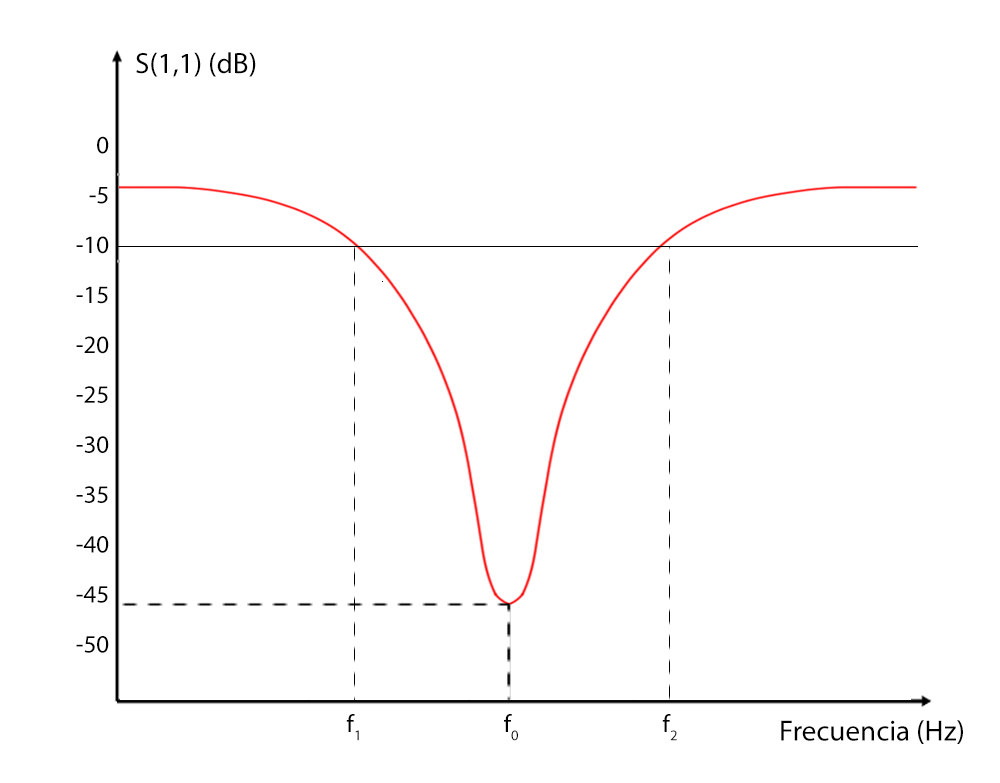
\includegraphics[width=12cm]{archivos/S}
        \caption{Representación gráfica de curva de parámetro S y ancho de banda de la antena}
        \label{fig:S}
\end{figure}

\par Además, dentro del rango de ancho de banda de la antena, se encontrará el mínimo de la curva del parámetro S. Este mínimo se definirá como la frecuencia de trabajo de la antena e intentaremos centrarlo siempre según las necesidades de nuestro diseño.


\section{Tipos de antenas}

\par En la práctica existen una gran variedad de tipos de antenas disponibles en el mercado, cada una de ellas es más conveniente según la aplicación para la que vaya a ser usada. Los parámetros descritos anteriormente serán fundamentales para diferenciar los tipos de antenas disponibles y saber identificar cual se adapta mejor a unas necesidades específicas. A continuación se mencionaran los tipos de antenas más comunes así como una breve descripción, resumen de las características principales y usos más comunes.

\subsection{Antenas de hilo}
\subsubsection{Antena dipolo}

\par Como se ha ido mencionado a lo largo del proyecto, el concepto más básico de antena se define como un dipolo (fig. \ref{fig:conjuntodipolo}). En la práctica un dipolo no es más que una linea de transmisión abierta cuyos extremos han de estar relacionados con la longitud de onda de la frecuencia a la que se quiera emitir para que la antena así posea resonancia. El patrón de radiación de un dipolo es, por lo general, omnidireccional en el plano H y con dos lóbulos en el plano E, obteniendo así un patrón de radiación tridimensional con forma toroidal cuyo radio interno es el diametro de los extremos del dipolo y con directividades entre los 1dB y 4dB. Según la longitud de los extremos abiertos del dipolo, el diagrama de radiación podrá ir variando e incluso llegaremos a observar la aparición de lóbulos secundarios y menores en ciertos múltiplos de la frecuencia a la que se quiera emitir (fig. \ref{fig:diagramadipolo}). Por ello, lo más común es que estos extremos midan en conjunto la mitad de la longitud de onda a la que se necesite emitir. A esta variación se le conoce como: Dipolo de media onda (Half-wave dipole).
\\
\begin{figure}[h]
    \centering
        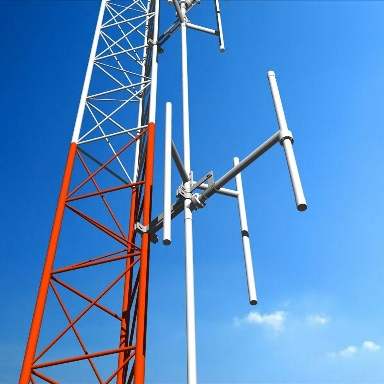
\includegraphics[width=0.6\textwidth]{archivos/dipolo/dipoloo}
        \caption{Conjunto de antenas dipolo \citep{Ideal-Antenas2008}}
        \label{fig:conjuntodipolo}
\end{figure}

\begin{figure}[h]
    \centering
        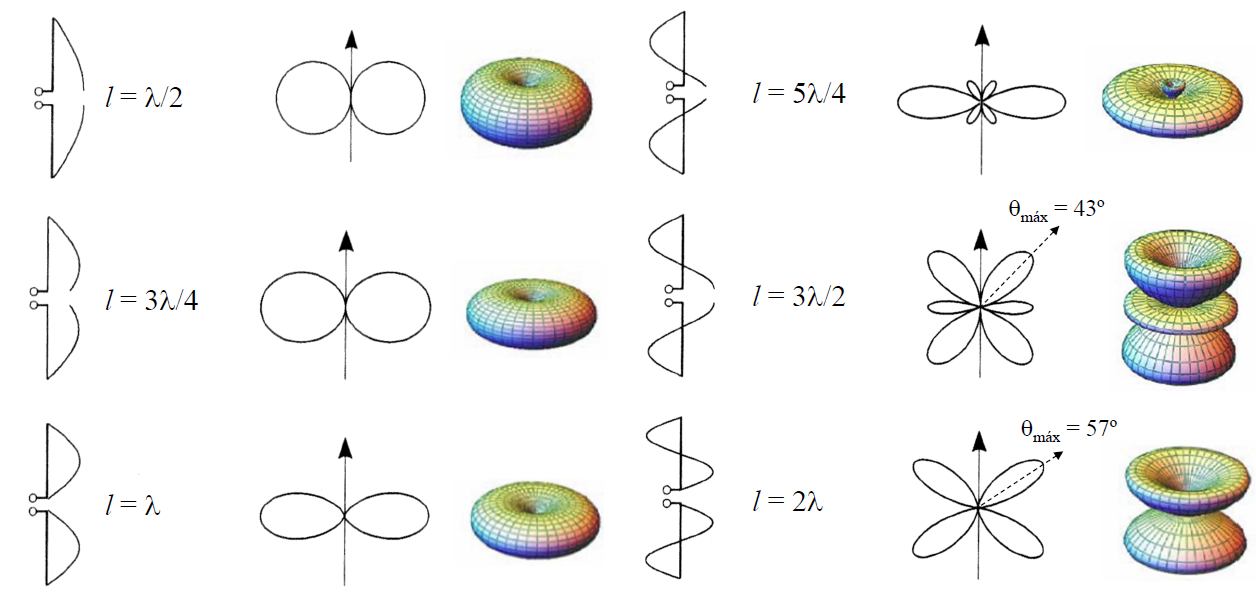
\includegraphics[width=\textwidth]{archivos/dipolo/radiaciones}
        \caption{Diagramas de radiación del dipolo según su longitud }
        \label{fig:diagramadipolo}
\end{figure}
\todo{referencia}
\par En su interior, a la frecuencia de resonancia, la distribución de corrientes muestra nulos en los extremos y un vientre en el centro y su polarización dependerá de la perspectiva según la localización del plano de masa: Si el campo eléctrico es perpendicular al plano de masa se observará una polarización lineal vertical, mientras que si se sitúa paralelo, se obtendrá una polarización lineal horizontal. La impedancia de estas antenas suele situarse sobre los 73$\Omega$.
\\
\par En la práctica, podemos encontrar derivaciones del dipolo según el caso de uso específico. Las modificaciones más usadas son:

\subsubsection{Antena Yagi-Uda}

La Antena Yagi-Uda (fig. \ref{fig:yagi}), inventada por \textit{Hidetsugu Yagi} y \textit{Shintaro Uda} en la cual un se agrupan un conjunto de elementos parásitos aumentando así la directividad y el ancho de banda de la antena. Esta antena se compone de tres partes principales: Los elementos directores, los reflectores y el dipolo. Los elementos directores son los encargados de incrementar la intensidad del campo en su dirección y reducirlas hacia el lado del reflector, por otro lado el reflector es el encargado de concentrar la radiación incidente en el dipolo. 
\\
\par Estos elementos parásitos no se conectan a  ninguna línea de transmisión sino que funcionan a través de inducción electromagnética mutua. En las antenas Yagi la ganancia puede llegar hasta los 40 dB por lo que es comúnmente usada para la recepción de transmisiones de \gls{tdt} y radio de \gls{fm} en hogares situados en las lejanías del repetidor local.



\begin{figure}[h]
\centering
	\begin{subfigure}[b]{0.45\textwidth}
    \centering
        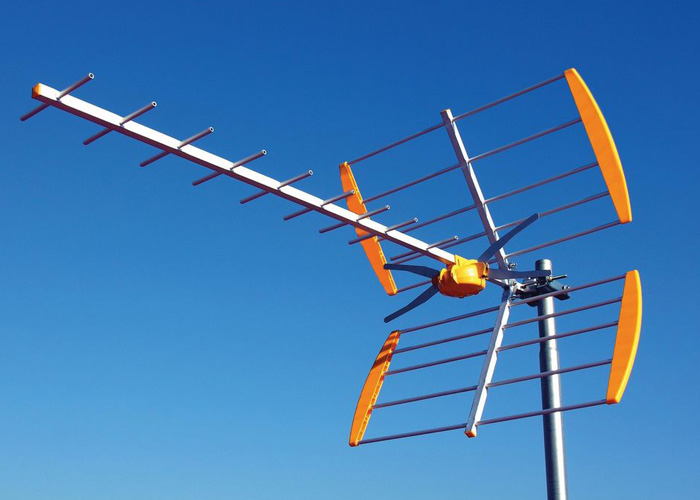
\includegraphics[width=\textwidth]{archivos/dipolo/yagi}
        \caption{Antena Yagi para recepción de TDT \citep{Pearce2010}}
        \label{fig:yagi}
	\end{subfigure}
~ % Añadir el espacio deseado, si se deja la linea en blanco la siguiente subfigura ira en una nueva linea
	\begin{subfigure}[b]{0.45\textwidth} % Espacio horizontal ocupado por la subfigura
	\centering
		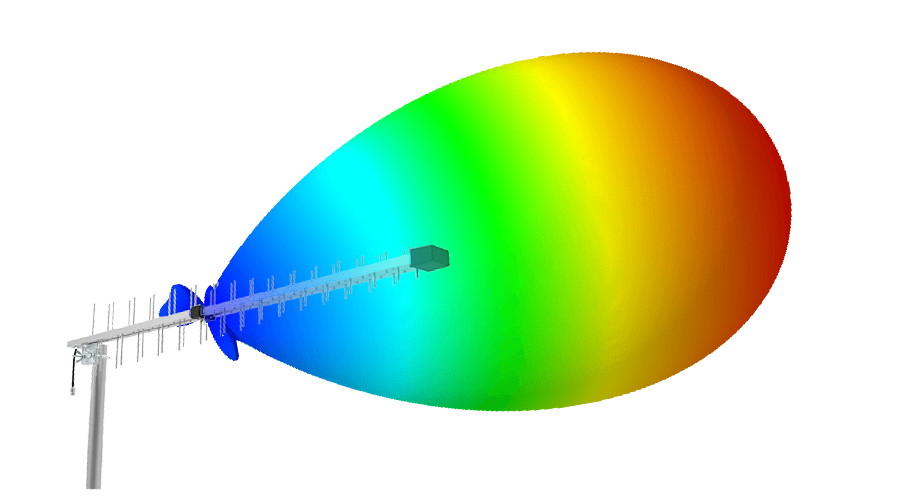
\includegraphics[width=\textwidth]{archivos/yagipat} % Tamaño de la imagen
		\caption{Diagrama de radiación común de antena yagi}
		\label{fig:yagirad}
	\end{subfigure}
\caption{Antenas Yagi}\label{fig:yagis}
\end{figure}

\subsubsection{Monopolo}

\par Otra variación conocida del dipolo es el monopolo, antena de Marconi o antena de cuarto de onda. En el, obviamos uno de los extremos del dipolo y lo sustituimos por un plano de masa lo cual hará la simulación electromagnética del extremo anulado del dipolo (fig. \ref{fig:monopolo}). El concepto original de Marconi para el monopolo se basaba en un cable de cuya longitud fuera un cuarto de la longitud de onda a la que se iba a transmitir ($\lambda$/4) situada sobre un plano de tierra que actuase como espejo electromagnético, obteniendo así una recreación de un dipolo de media onda.
\\
\par A efectos prácticos, obtendremos un dipolo de media onda con una impedancia igual a la mitad del dipolo original. El diagrama de radiación contendrá solo la parte superior del toroide obtenido en el dipolo pero con el doble de intensidad de radiación que en este, es decir, con una ganancia 3dB mayor.
\\
\begin{figure}[h]
    \centering
        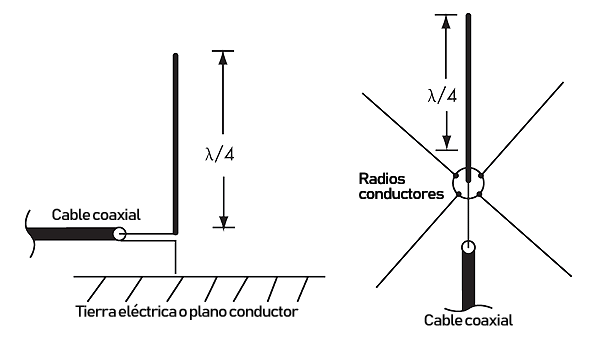
\includegraphics[width=0.7\textwidth]{archivos/monopolo/monoesquema}
        \caption{Esquema de instalación de un monopolo. \citep{Frenzel2013}}
        \label{fig:monopolo}
\end{figure}

\par La polarización de la antena será siempre lineal vertical, puesto que el plano de masa comúnmente usado está instalado sobre el suelo terrestre. Esta masa debe ser buena conductora ya que es de vital importancia para la correcta reflexión de las \gls{oem} procedentes del extremo radiante. Estas antenas suelen ser instaladas sobre los techos de barcos, donde el agua actúa sobre una perfecta masa conductora, o sobre el techo de los coches, que al ser metálico, también ayuda a la correcta reflexión de las \gls{oem}. 
\\
%\begin{figure}[h]
%    \centering
%        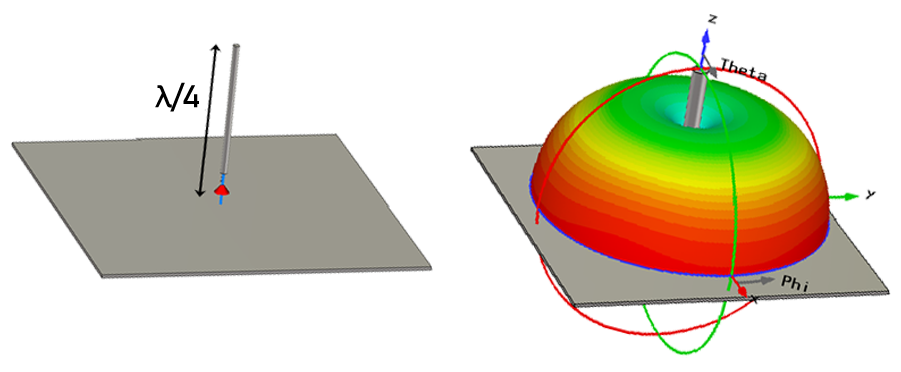
\includegraphics[width=14cm]{archivos/monopolo/fig3}
%        \caption{Diagrama de radiación 3D de un monopolo}
%        \label{fig:monopolorad}
%\end{figure}

\par En caso de que la antena se instale sobre superficies no conductoras, existen distintas alternativas como humedecer la tierra o instalar radios conductores. Los radios son tiras metálicas dispuestas concentricamente al rededor del monopolo. Cuanto mayor sea la longitud de las tiras, mejor simulación del dipolo obtendremos. Unas tiras muy pequeñas resultaran en un diagrama de radiación muy separado del suelo.
\\
\par La ventaja principal de estas antenas es la reducción a la mitad de la longitud necesaria para el funcionamiento de la antena. En situaciones como las antenas de los coches, barcos o aviones, es importante reducir al máximo la longitud de las antenas para que no afecten al uso del vehículo. Otro uso muy importante es para la baja frecuencia, por ejemplo, en transmisiones de \gls{am}, donde la frecuencia de transmisión ronda entre los 500 y 900 KHz, la longitud de la antena dipolo de media onda necesaria para la retransmisión sería de entre 100 y 200 metros, mientras que con el monopolo, estas distancias se reducen a la mitad, facilitando su construcción, instalación y mantenimiento (fig. \ref{fig:monopoloam}).

\begin{figure}[h]
    \centering
        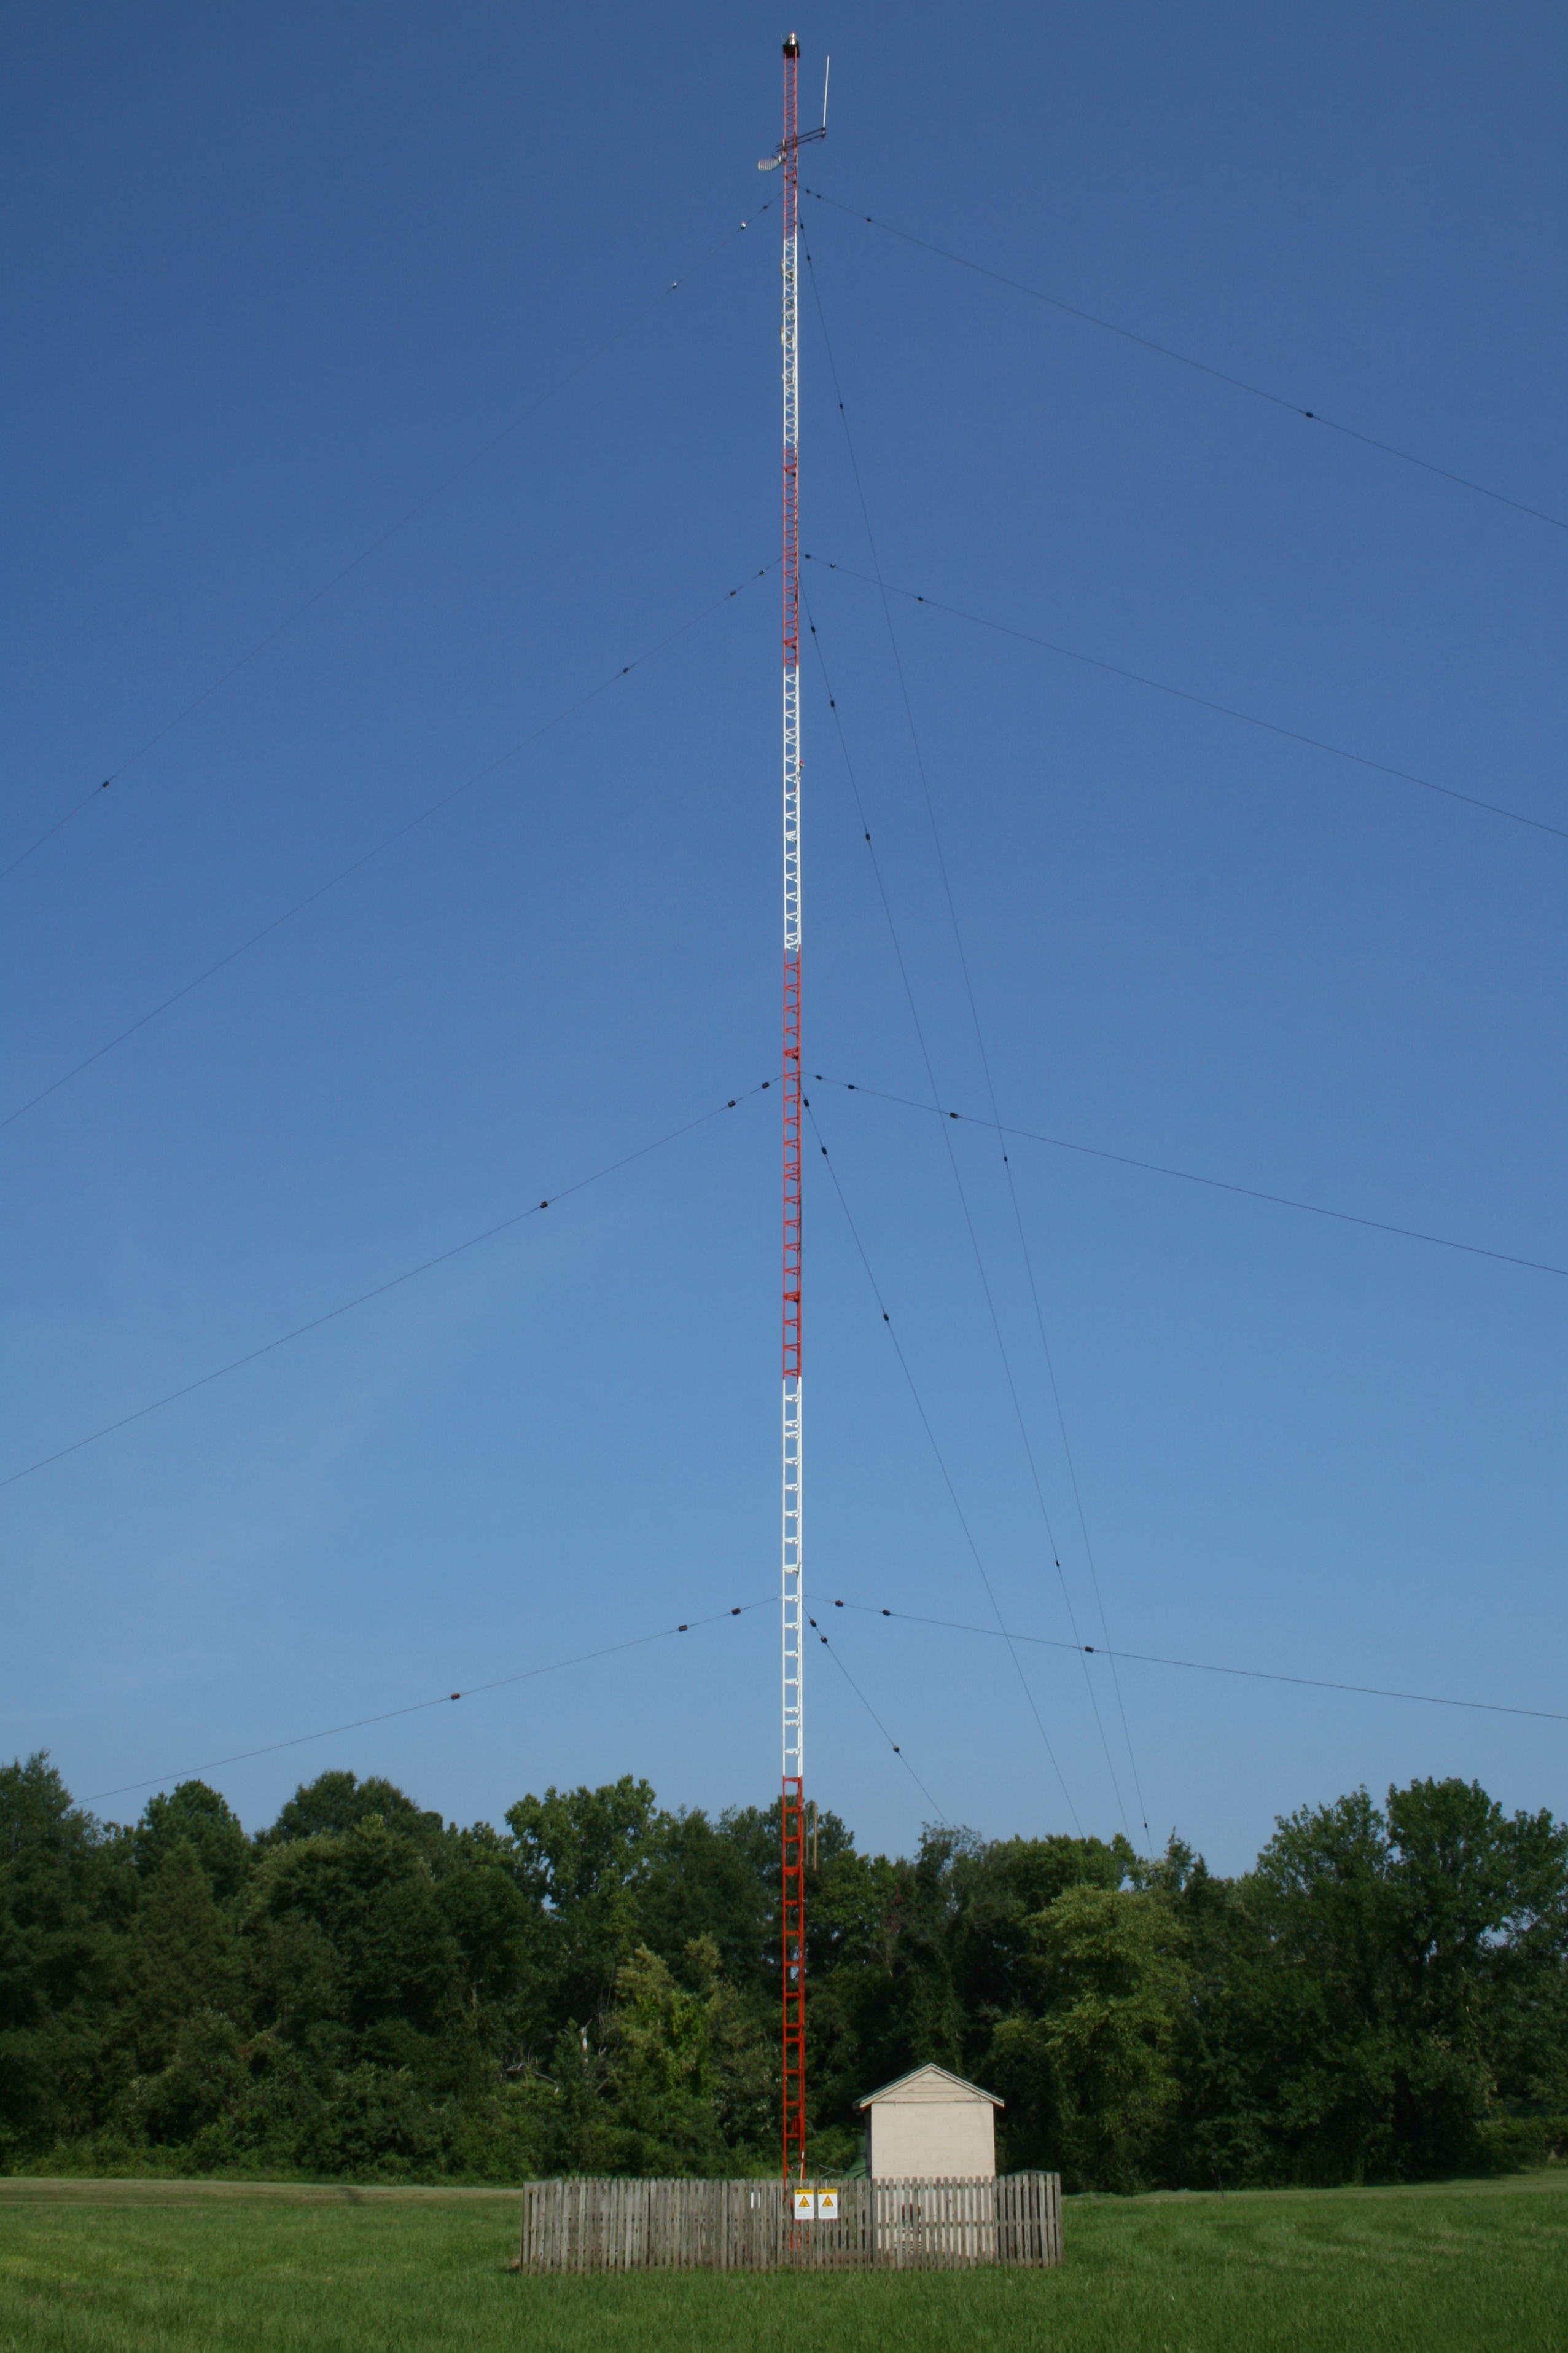
\includegraphics[width=0.4\textwidth]{archivos/monopolo/monopolo}
        \caption{Monopolo para transmisión de AM. \citep{Sagdejev2008}}
        \label{fig:monopoloam}
\end{figure}

\subsection{Antenas de apertura}
\subsubsection{Bocinas}

\par Las antenas de tipo bocina se caracterizan por su forma cónica o rectangular parecida a la de un altavoz. Su uso se remonta a finales del año 1800, pero este tipo de antenas adquirió popularidad durante la segunda guerra mundial (fig. \ref{fig:horn}). La diferencia de estas antenas con respecto a las antenas de tipo cable es que estas son alimentadas mediante una guía de onda. Una guía de onda es una estructura física capaz de transportar modos electromagnéticos en su interior. Suelen usarse para la guiado de emisiones de alta frecuencia, más en concreto de microondas debido a su baja atenuación en estas magnitudes. En el interior de las guías de ondas, las \gls{oem} viajan confinadas de modo que no hay pérdidas por radiación en el espacio y se consiguen evitar las interferencias electromagnéticas externas durante su guiado.
\\
\par Por lo general, las bocinas son usadas para la radiación de microondas y tienen un papel importante en campos como la radio astronomía o seguimiento satelital, además de ser usado junto a otros elementos como reflectores o lentes y sirven como estándar universal para la calibración de antenas de alta ganancia. En el caso de las bocinas piramidales, las dimensiones de los lados de la apertura definen qué plano de radiación es más efectivo en la antena. Si la longitud mayor es la del plano horizontal se denominarán bocinas de plano H, y en el plano vertical, bocinas de plano E. El modo de propagación siempre es el \gls{te} 10. En el caso en el que la bocina sea circular, el modo de propagación será el TE11.
\\
\par La directividad de este tipo de antenas es una de sus principales ventajas siendo esta muy moldeable solo variando las dimensiones de la apertura de la bocina. Su principal desventaja llega en su eficiencia, que suele rondar entre el 50\% y el 60\%.
\begin{figure}[h]
    \centering
        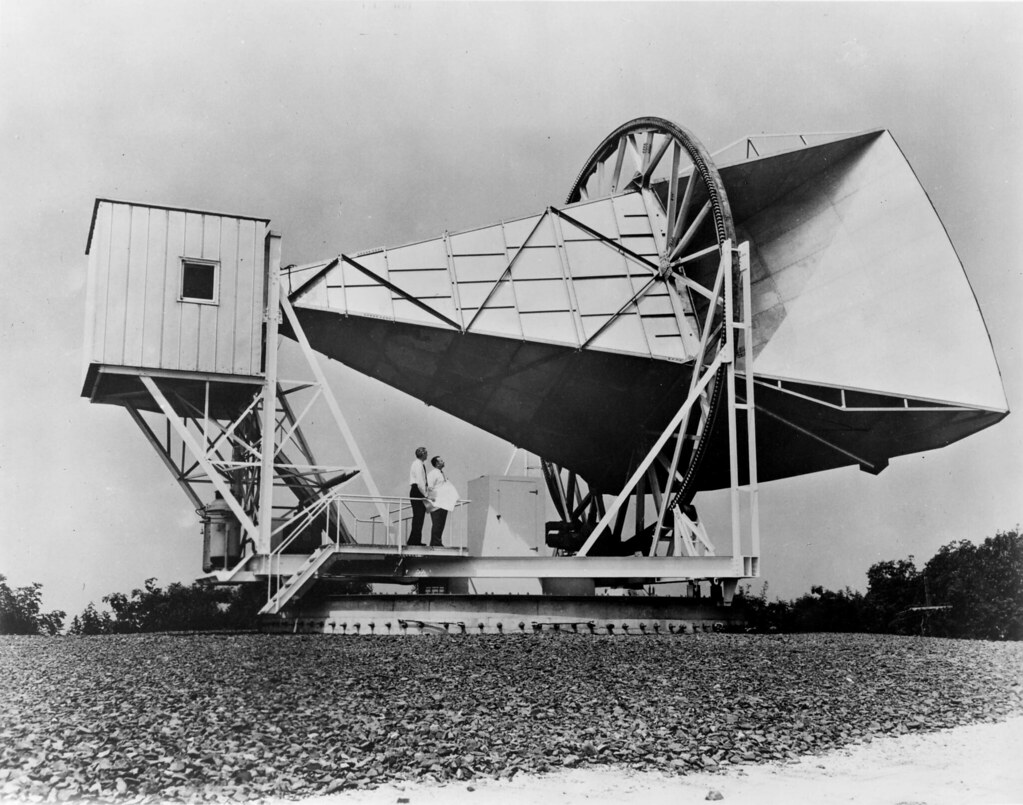
\includegraphics[width=0.8\textwidth]{archivos/horn}
        \caption{Bocina para comunicación satelital construida en 1959 por los laboratorios Bell. \citep{NASA1962}}
        \label{fig:horn}
\end{figure}

\subsubsection{Reflectores}

\par Las antenas reflectoras han sido usadas desde el descubrimiento de la propagación electromagnética en 1888 por \textit{Hertz}, quien realizó sus primeros experimentos con reflectores en forma de cilindro parabólico. Durante el perido de la segunda querra mundial, este tipo de antenas fueron estudiadas para numerosas aplicaciones radar. Con el paso del tiempo, este tipo de antena son muy comunes en ámbitos como la radio astronomía, comunicaciones por microondas, y seguimiento satelital. Aunque los reflectores puedan tomar cualquier forma, es común observarlos en formas planas, cónicas o curvas, en especial en forma parabólica. 
\\
\par Aunque los reflectores se puedan diseñar y analizar mediante técnicas del campo de la óptica como la óptica geométrica y el trazado de rayos, lo más común es usar la teoría geométrica de la difracción o \gls{gtd}. Cada tipo de reflector es capaz de ofrecer una serie de características diferentes a la antena que pueden ser convenientes según el uso final de esta, como el área efectiva de radiación, la relación delante/atrás, o los diagramas de radiación y ganancias.
\\
\par En la actualidad uno de las superficies reflectoras más usada es la curva parabólica, o como se conoce popularmente, antena parabólica. Esta antena se caracteriza por su superficie reflectora, una parábola de revolución. Lo interesante de esta geometría es su capacidad de concentración de los haces electromagnéticos sobre el foco de la parábola. Existen distintos tipos de antenas parabólicas según el diseño de la posición del foco respecto a la superficie reflectora:

\begin{itemize}
	\item \textbf{Parabólica de foco centrado: }La superficie reflectora es parabólica y el alimentador esta sobre el foco.
	\item \textbf{Parabólica off-set: }La superficie reflectora es una sección del reflector parabólico normal y se encuentra desplazado con respecto al foco. Este variación de antenas parabólicas son más eficientes que las de foco centrado puesto que el alimentador no hace sombra sobre la superficie reflectora
	\item \textbf{Parabólica Cassegrain: }En esta variación, encontramos dos superficies reflectoras: Una superficie parabólica cóncava y una superficie hiperbólica convexa. Con este sistema se consigue un alto nivel de ganancia, lo que lo hace útil para aplicaciones astronómicas.
\end{itemize}

\par Por lo general, este tipo de antenas se caracterizan por su patrón de radiación, en donde la mayor parte de la energía radiada se concentra sobre un lóbulo principal estrecho. La potencia restante se disipa en forma de lóbulos secundarios en otras direcciones. Además, podemos encontrar un lóbulo trasero debido al efecto spillover, es decir, la parte de la radiación procedente del alimentador que sobresale al reflector, el cual puede ser reducido añadiendo material capaz de absorber microondas o aumentando el tamaño del reflector. 


\begin{figure}[h]
    \centering
        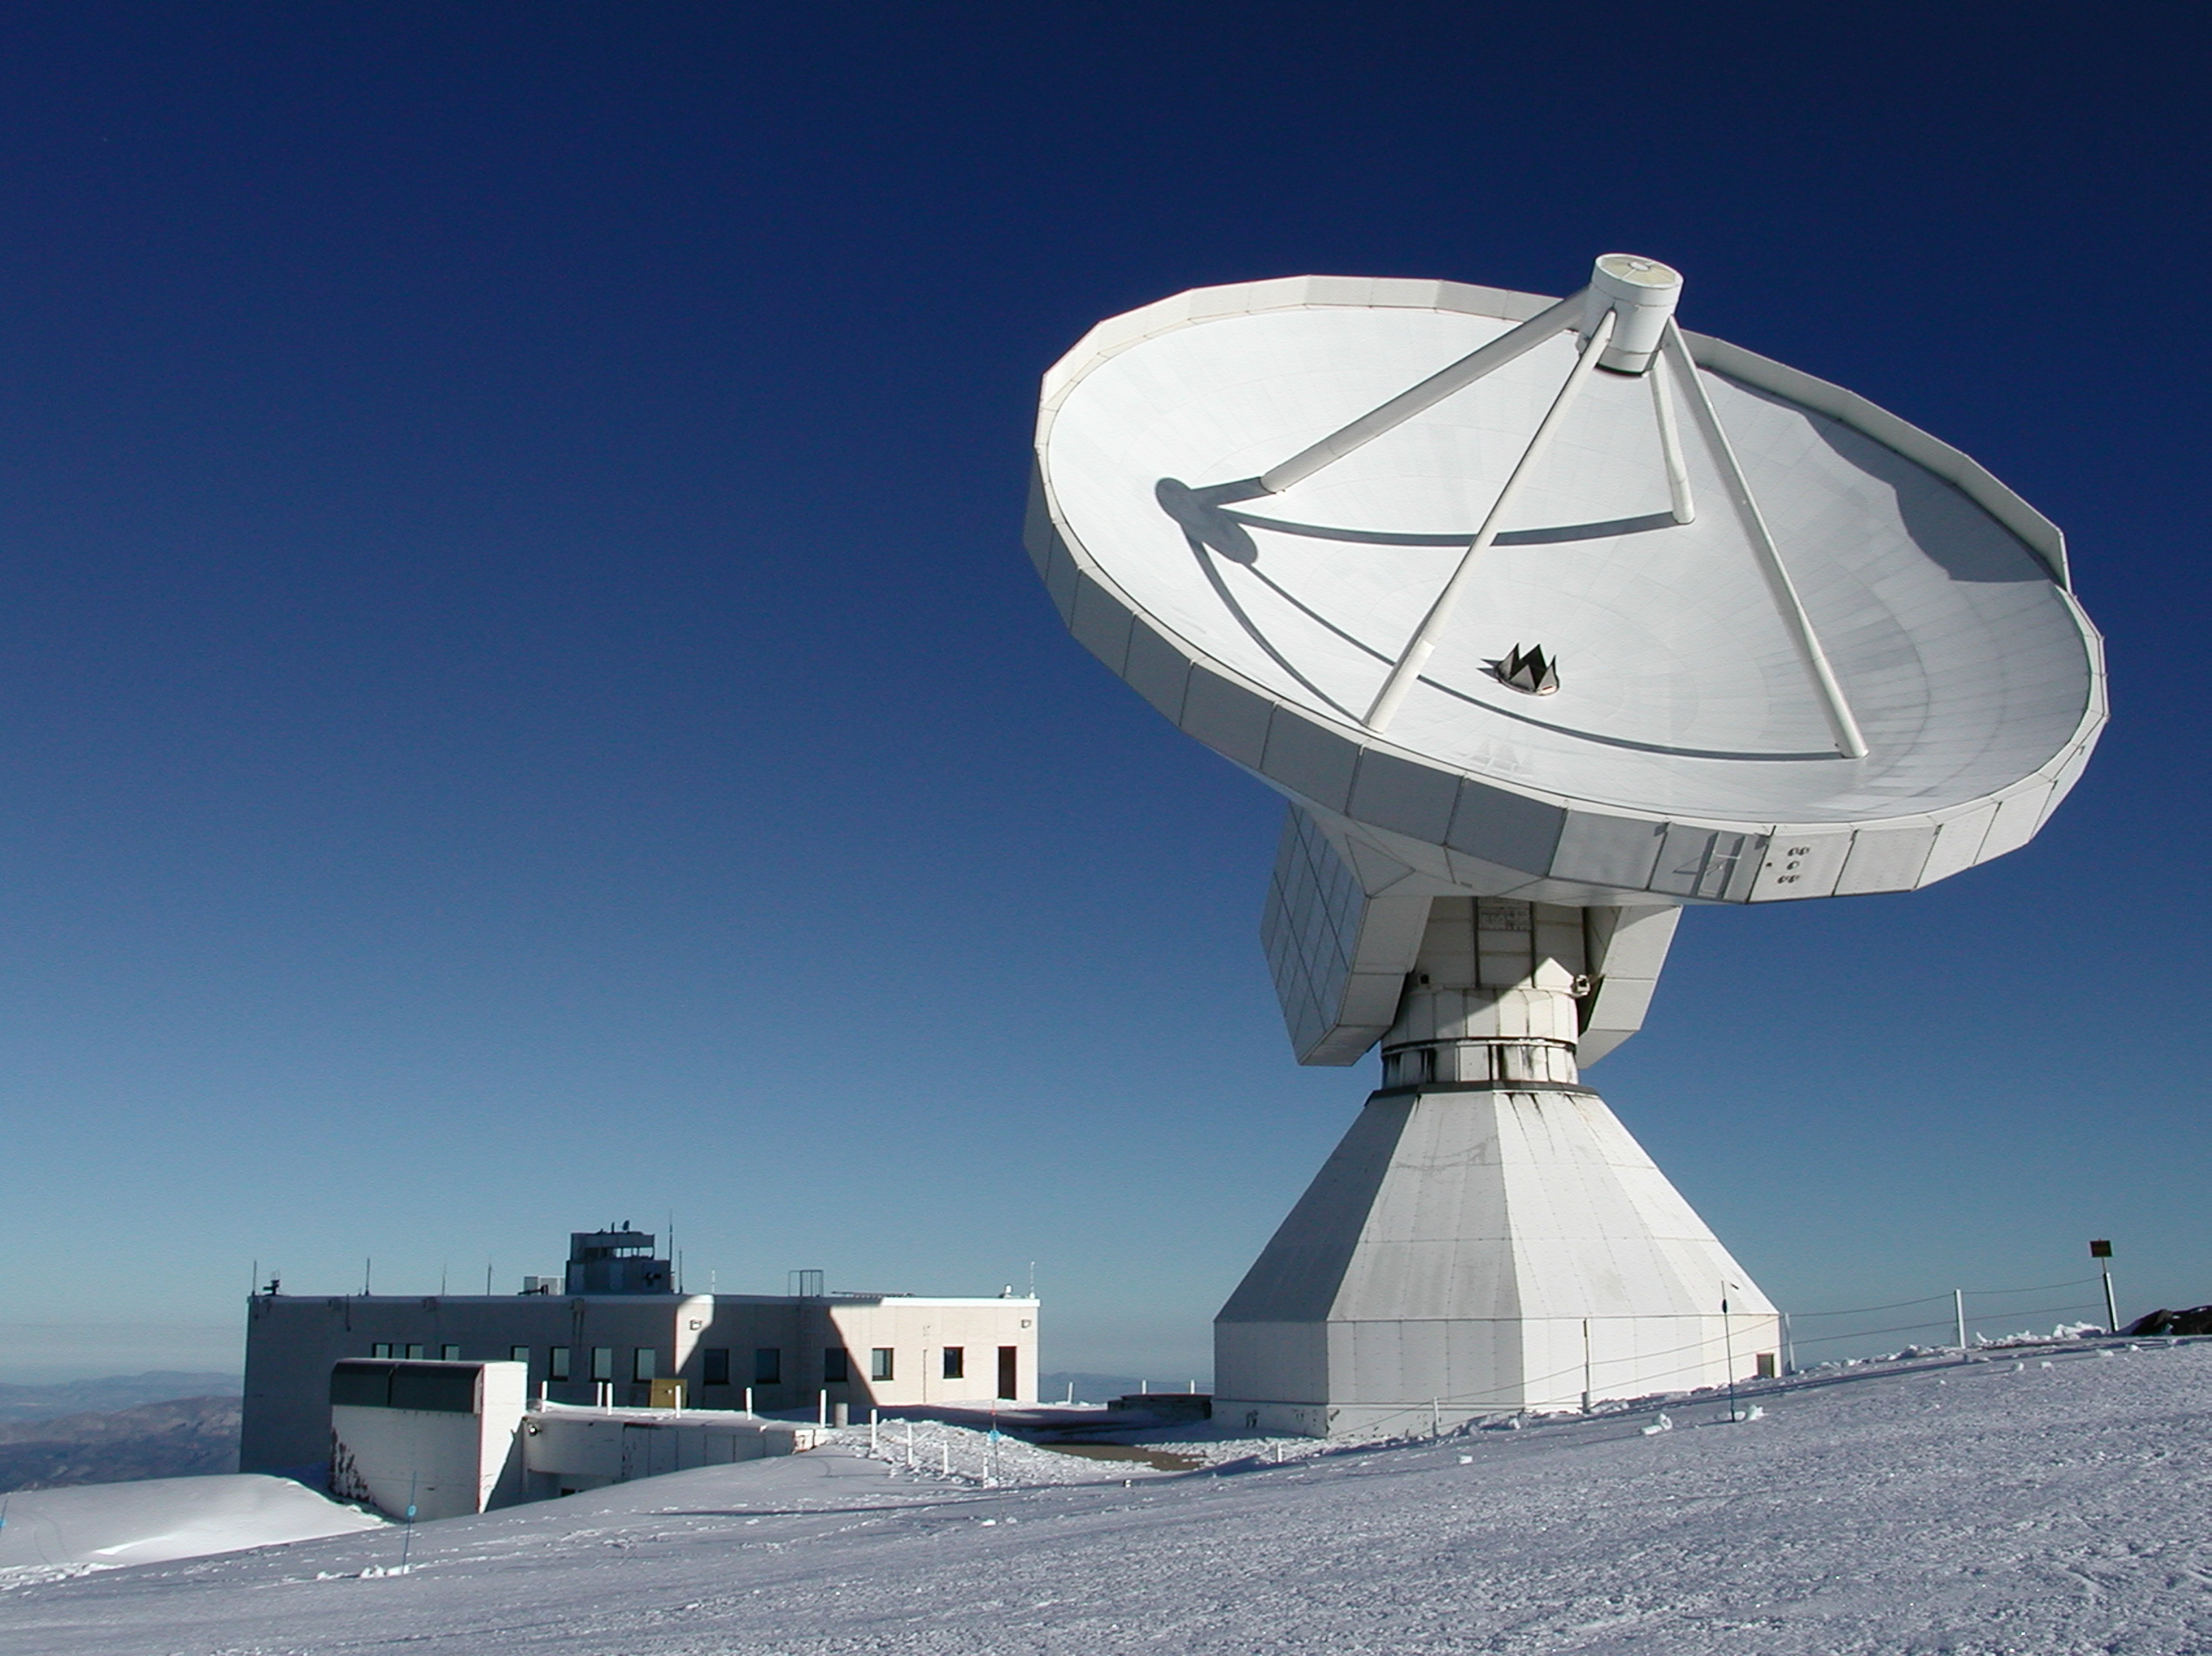
\includegraphics[width=0.8\textwidth]{archivos/parab}
        \caption{Antena parabólica del IRAM en Sierra Nevada, parte del proyecto Event Horizon para capturar la primera fotografía de un agujero negro. \citep{MICIU2019}}
        \label{fig:parabolica}
\end{figure}

\par En la actualidad podemos encontrar este tipo de antenas comúnmente en balcones y tejados en los edificios de las ciudades puesto que durante décadas este tipo de antenas han sido usadas para la recepción de televisión por satélite. También son muy usadas para radio enlaces, ofreciendo servicios de internet WiMax, operadores VoIP o comunicaciones rurales. Finalmente, otra de las aplicaciones más importantes de los reflectores parabólicos se encuentra en la radio astronomía, donde estas antenas son instaladas en conjunto formando arrays. 
\\
\par Un array de antenas es un conjunto de estas diseñadas para trabajar de forma conjunta y así obtener resultados que con una sola antena sería imposible de conseguir. El último ejemplo más destacado lo encontramos con la fotografía del primer agujero negro por parte del proyecto \textit{Event Horizon Telescope}. En este proyecto se usaron varios radio telescopios instalados en distintas partes del mundo como el Alfonso Serrano en Mexico, el South Pole Telescope en el Polo Sur, el James Clerk Maxwell Telescope en Hawai o el \gls{iram} (fig. \ref{fig:parabolica}) 30-m en España. La finalidad de la utilización de estos telescopios es la de actuar como un solo radio telescopio cuyo diámetro sería imposible de alcanzar mediante uno solo.

\subsection{Antenas Microstrip}

\par Las antenas microstrip son una extension de las lineas de transmisión por tecnología microstrip cuyo extremo queda abierto y con unas dimensiones específicas de forma que el parche disipe energía en forma de radiación. Este tipo de antenas serán las utilizadas para el desarrollo de este estudio debido a sus características de construcción y sus capacidades técnicas y serán analizadas a fondo en el capitulo \ref{antenasmicrostrip}.
\vfill

\begin{figure}[h]
     \centering
     \begin{subfigure}[b]{\textwidth}
         \centering
         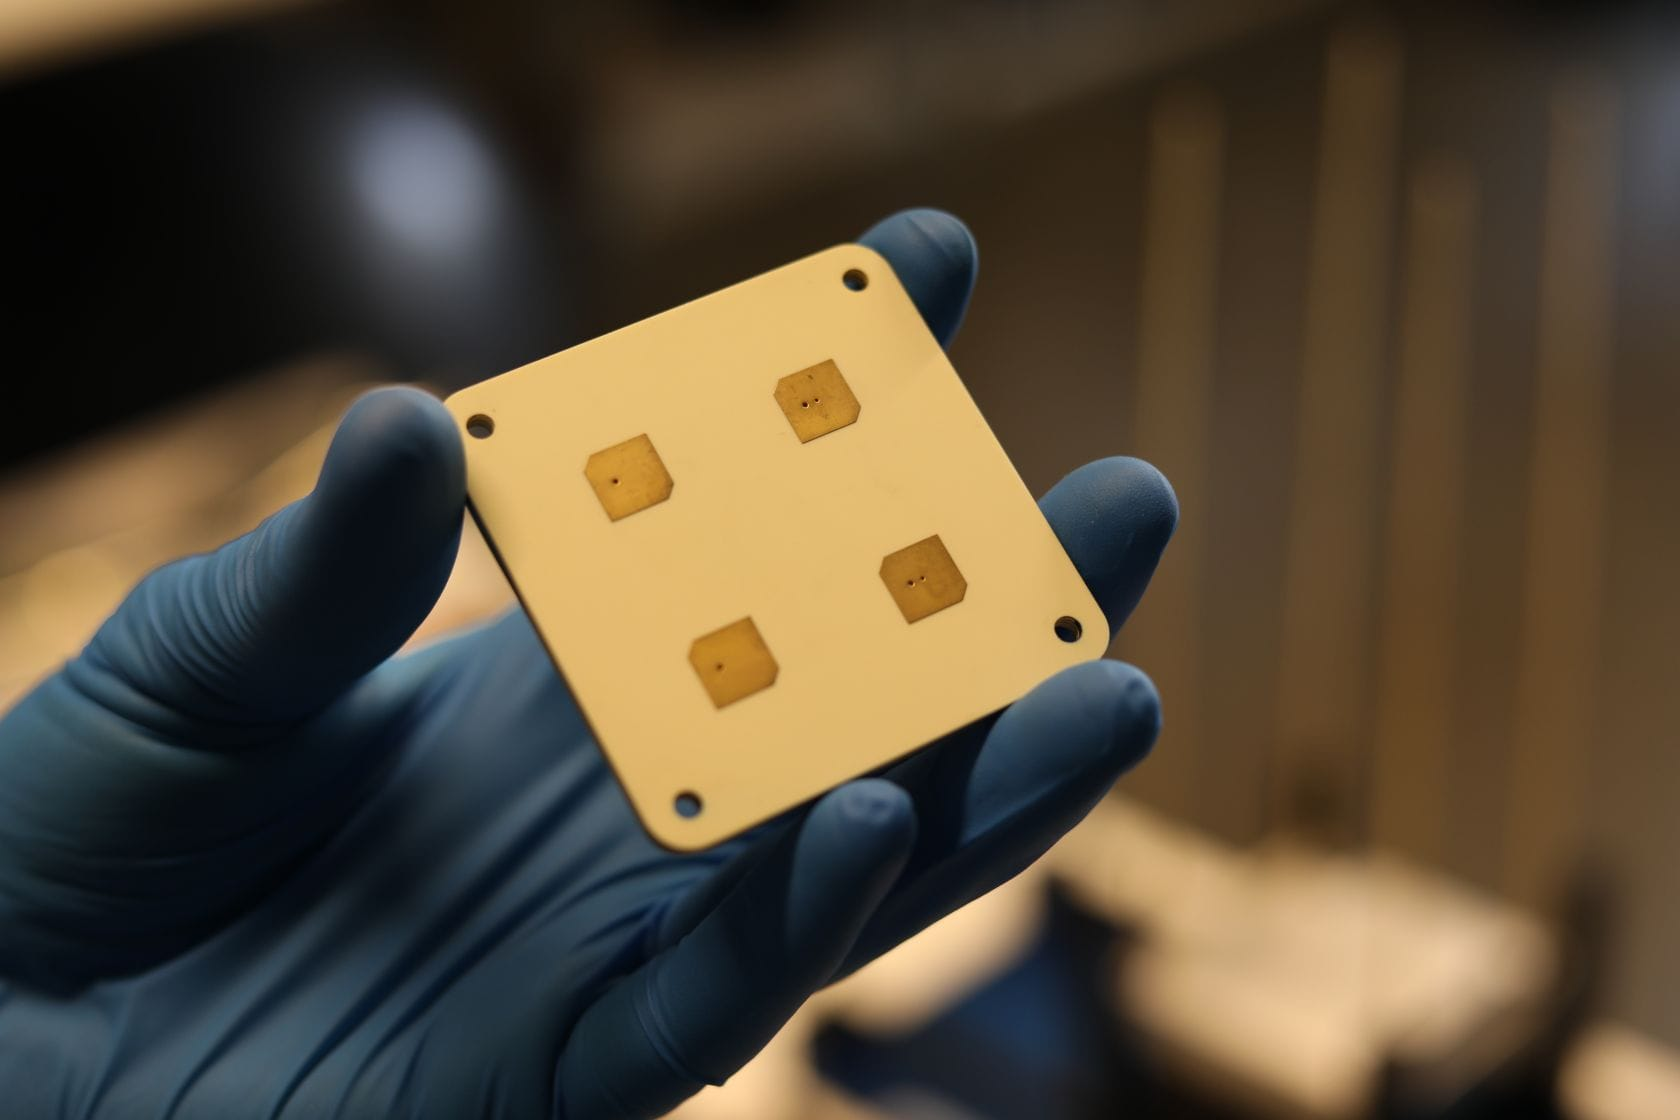
\includegraphics[width=0.7\textwidth]{archivos/enduro1}
         \caption{Vista delantera}
         \label{fig:endur1}
     \end{subfigure}
\vfill
     \begin{subfigure}[b]{\textwidth}
         \centering
         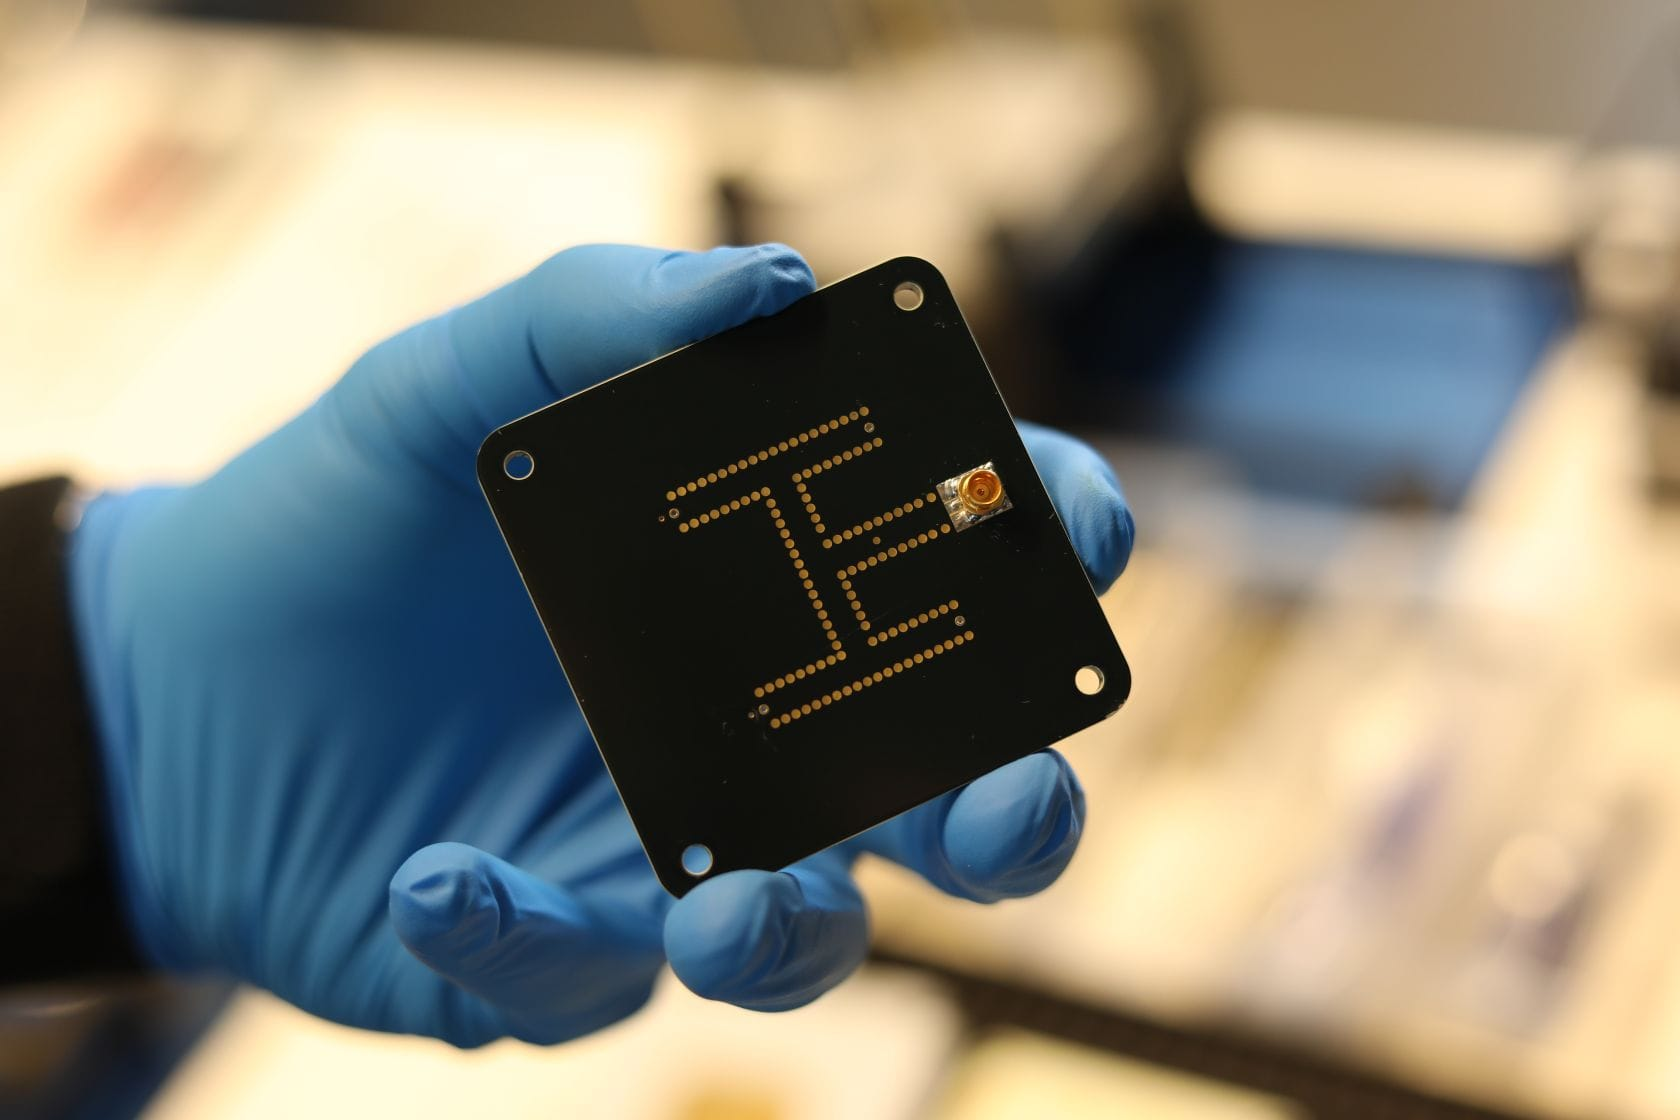
\includegraphics[width=0.7\textwidth]{archivos/enduro2}
         \caption{Vista trasera}
         \label{fig:endur2}
     \end{subfigure}

        \caption{Array de antenas microstrip para aplicaciones satelitales. \citep{Endurosat2018}}
        \label{fig:endur}
\end{figure}
\vfill
